\usepackage{placeins}
\usepackage{float}
\documentstyle[12pt,graphicx]{article}
\pagestyle{plain}
\baselineskip 18pt
\textwidth 6.5in
\textheight 7.8in
\oddsidemargin 0.1in
\evensidemargin 0.1in
\topmargin 0.3in
\parindent 0pt
\renewcommand{\thesubsection}{\thesection.\alph{subsection}}
\newcommand{\beq}{\begin{equation}}
\newcommand{\eeq}{\end{equation}}

\begin{document}

\title{Homework 2 - Solving ODEs by  Runge-Kutta Method}
\author{Quynh Nguyen}
\maketitle


Note: The zip folder include main c++ code in /comp/hw2/ and ROOT plot code in /root/macros. Code is compiled in g++ (clang) in Mac OSX. 



\section{Problem 1}
\paragraph{}
 Let \( \frac{du}{d\phi} \) = v and \( \frac{d^2u}{d{\phi}^2} \) = dv then the given equation of motion (1) becomes the system of equation:



\beq
\frac{dv}{d\phi}\ + u = \alpha + \beta u^2
\label{dv}
\eeq

\beq
\frac{du}{d\phi}\ = v
\label{v}
\eeq


with $\frac{GM}{h^2} = \alpha $ and $\frac{3GM}{c^2} = \beta $. This system of first-order ODE equation can be solved by Runge-Kutta method. 
Let $ \vec{y}=(u,v) $ the system can be written as:
\beq
\frac{d\vec{y}}{d\phi}\ = \frac{d}{d\phi} \left(
\begin{array}{c}
u\\
v\\
\end{array}
\right) = \left(
\begin{array}{c}
v\\
\beta u^2 - u + \alpha\\
\end{array}
\right)
= \vec{f}(u,v,\phi})
\label{sys}
\eeq

Apply Runge-Kutta method with initial condition $\vec{y}(0)= \left( \begin{array}{c}
a(1+e)\\
0\\

\end{array}  \right)$ where a is the major axis and e is the eccentricity, thus u(0) is the inverse of the perihelion.

\subsection{Code implementation}
\paragraph{}
Please see the attached file "comp/hw2/problem1.cc" for the code.

\subsection{Mercury orbit around the Sun}
\paragraph{}
  The close orbit is shown by plotting the radius and $\phi$ in polar coordinate as in Figure (\ref{polar}).


\begin{figure}[!htbp]
\begin{center}
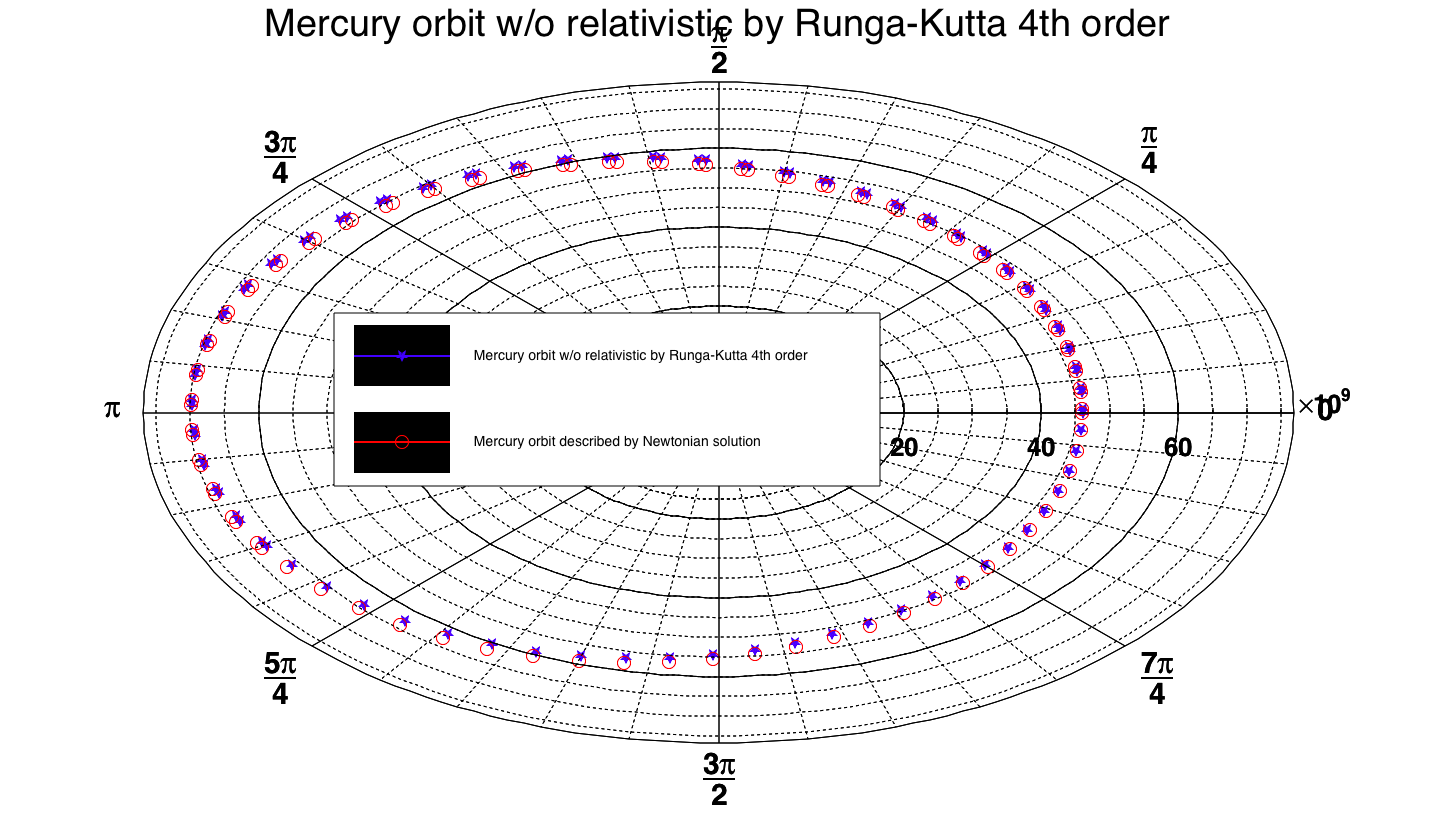
\includegraphics[width=0.8\textwidth]{1_b_polar_1.png}
\caption{Close orbit produce by Runge-Kutta without relativistic term }
\label{polar}
\end{center}
\end{figure}

This this plot, the relativistic term $ \beta$ is turned off. The Runge-Kutta solution (blue) and Newtonian exact solution (red) are plotted together for different step sizes in Figure (\ref{1b10}) (\ref{1b100}) and (\ref{1b500}) .It is obviously that, the more steps used, the more overlapping between the two solutions.

\begin{figure}[!htbp]
\begin{center}
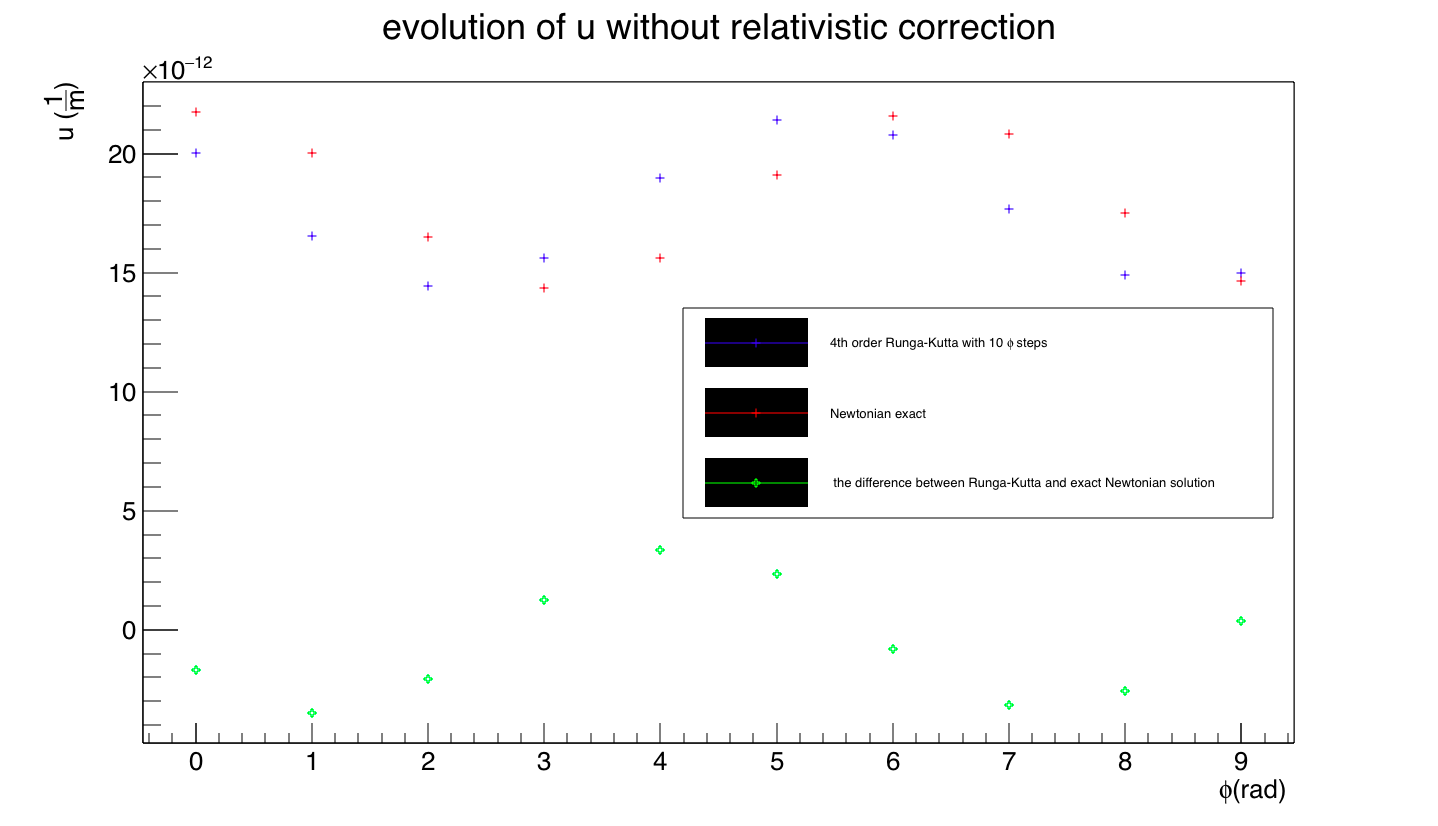
\includegraphics[width=0.8\textwidth]{1_b_n10.png}
\caption{Comparing u with newtonian solution at 10 time steps}
\label{1b10}
\end{center}
\end{figure}

\begin{figure}[!htbp]
\begin{center}
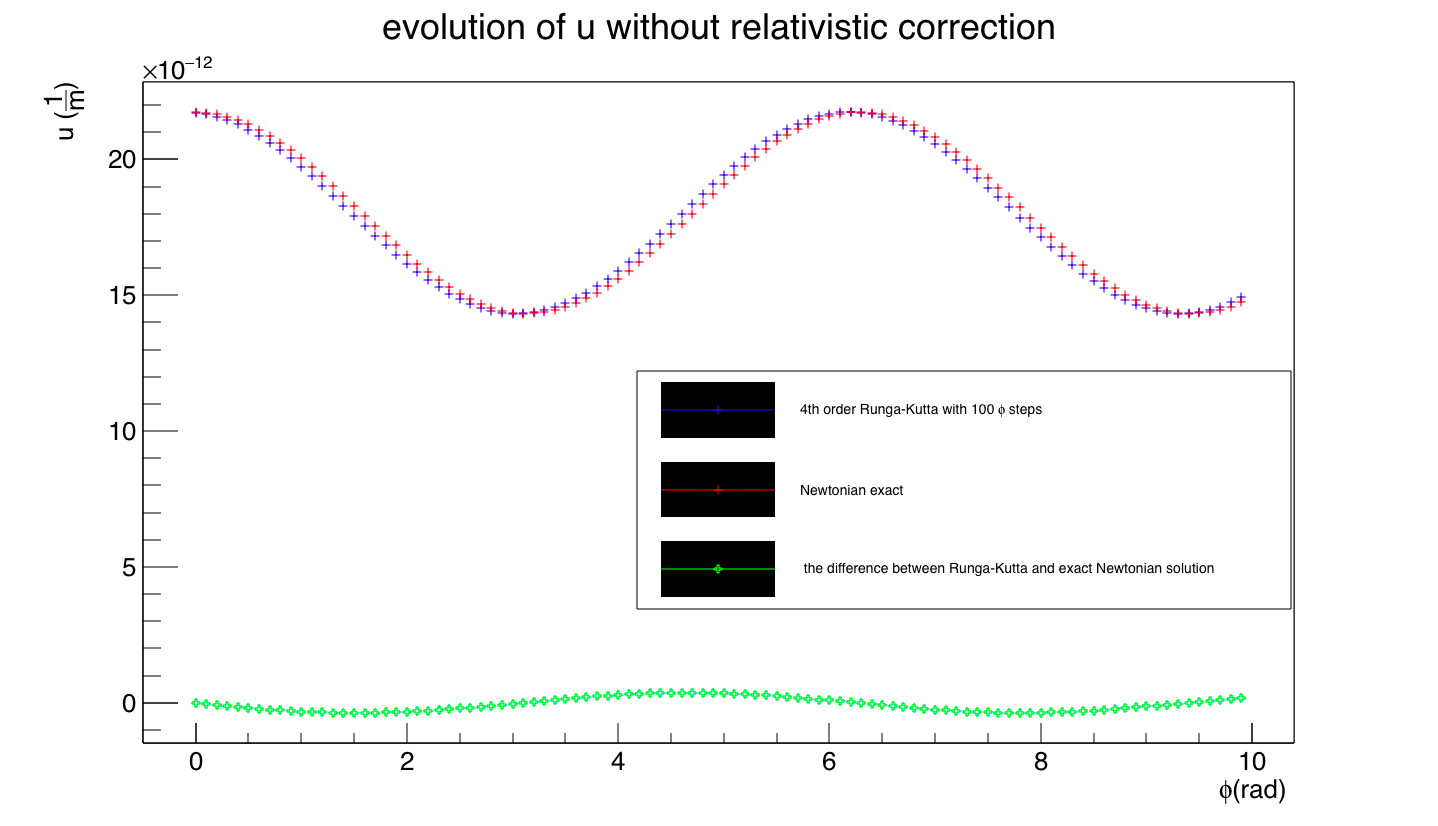
\includegraphics[width=0.8\textwidth]{1_b_n100.png}
\caption{Comparing u with newtonian solution at 100 time steps}
\label{1b100}
\end{center}
\end{figure}


\begin{figure}[!htbp]
\begin{center}
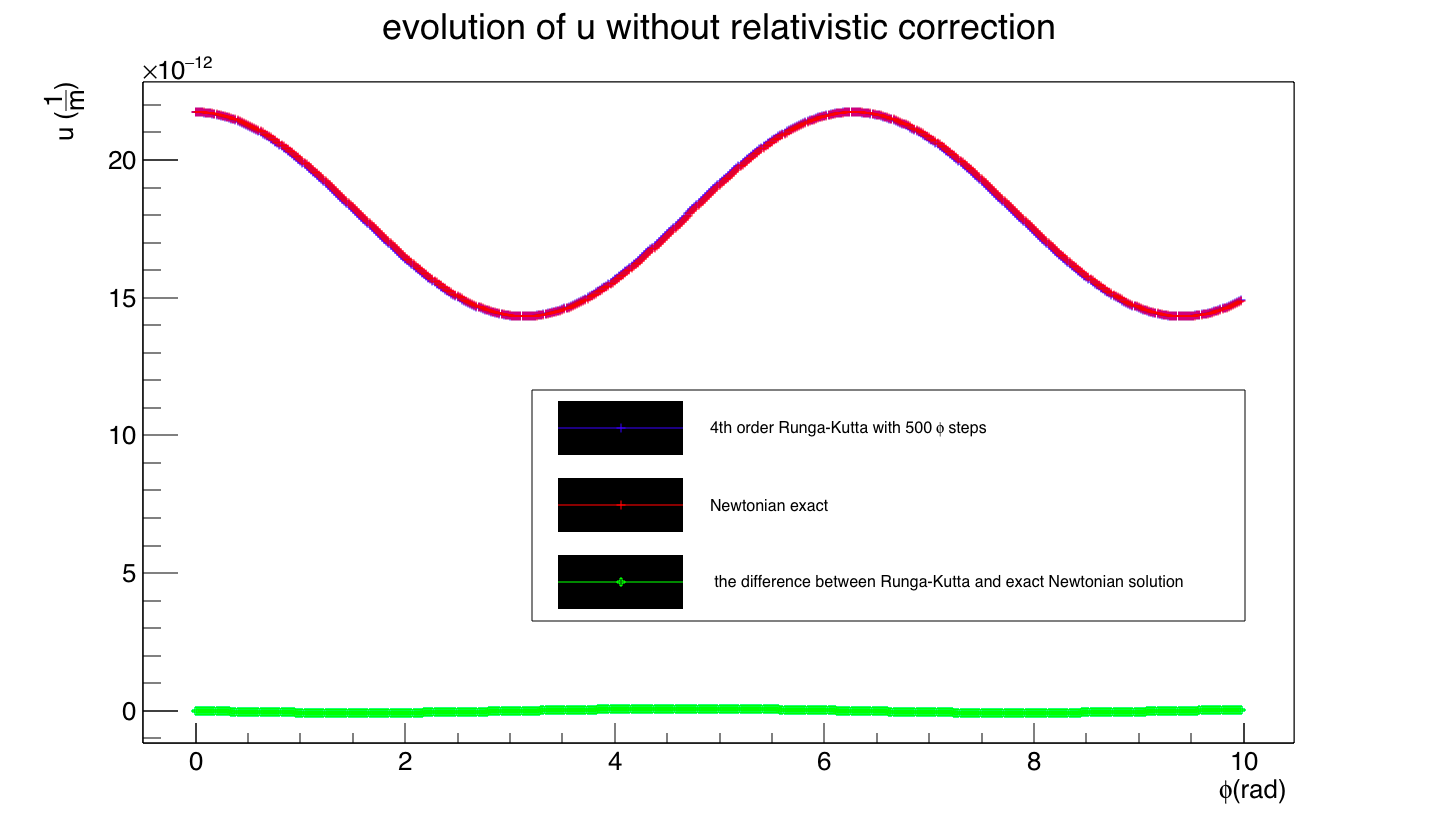
\includegraphics[width=0.8\textwidth]{1_b_n500.png}
\caption{Comparing u with newtonian solution at 500 time steps}
\label{1b500}
\end{center}
\end{figure}


\FloatBarrier
\subsection{The perihelion shift}
\paragraph{}
The relativistic term $ \beta $ is now included. To find the shift in $\delta \phi $, the Runge-Kutta program runs for just pass  one period with initial position as in section 1.b. The number of step was set to $10^{7} $ for high precision and numerical values are set at high precision.

\paragraph{}
The initial point of ( $\phi$ , u) is (0,1/perihelion) = (0, 2.17382199142713e-11).
Three points nearest the maximum of u were fit into a quadratic u = $a\phi^2+b\phi+c$ which first derivative was used to find the value of $\phi$ at maximum of u, i.e the perihelion.
$\phi_{perihelion}$ found to be 6.283184785 
Thus 

\begin{equation}
\Delta \phi_{shift} = ( 6.283184785- 2 \times \Pi ). \frac{rad}{period}   \times \frac{180}{\Pi} .\frac{degree}{rad} \times  \frac{100}{0.241 }.\frac{period}{century}  \simeq 44.7 \frac{arcsecond}{century}
\end{equation}
\paragraph{}
This is approximately equal to the magnitude to the famous pertubative result. The result could be improved by increasing time steps or fitting with more points.

\section{Problem 2}
\subsection{Equation of orbit}
\paragraph{}
The equation of motion of particle mass m subjected to central force f(r) in polar coordinate is: 
\beq 
m\ddot {\vec{r}} = f(r) \vec{e_r} 
\eeq 
while taking derivative in polar coordinate give $\ddot {\vec{r}} $ = ( $\ddot r$ - r$ \dot {  \phi ^2  }) \vec{e_r} + ( 2 \dot{r} \dot{\phi} + r\ddot{\phi})  \vec{e_{\phi}$
Thus the component-wise equation of motion are:
\beq
m(\ddot{r}-r\dot{\phi^2}) = f(r)
\label{radial}
\eeq

\beq
m(2\dot{r} \dot{\phi} +r\ddot{\phi}) =0
\label{l}
\eeq
from equation \ref{l} :
\beq
\frac{d}{dt}(r^2\dot{\phi}) = 0
\eeq

or $r^2\dot{\phi}$ = h = constant. Let u = $\frac{1}{r}$ then $ \dot{r}=-\frac{1}{u^2}\dot{u}= -\frac{1}{u^2}\dot{\phi}\frac{du}{d\phi} = -h \frac{du}{d\phi}$. Differentiate this gives:
\beq
\ddot{r} = -h \frac{d}{dt} \frac{du}{d\phi} = -h \frac{d\phi}{dt}\frac{d}{d\phi}\frac{du}{d\phi} = -h\dot{\phi}\frac{d^2u}{d\phi^2}  = - h^2 u^2 \frac{d^2u}{d\phi^2}

\eeq
substituting r, $\dot{r}$ and $\dot{\phi}$ back to equation (\ref{radial}) 
\beq
m \big( -h^2u^2 \frac{d^2u}{d\phi^2}-\frac{1}{u}h^2 u^4 ) = f(u^{-1})
\eeq

simplify, the orbital equation for a particle moving under a central for is
\beq
\frac{d^2u}{d{\phi^2}}\ + u =  \frac{1}{mh^2u^2}f(u^{-1})
\label{central}
\eeq
plug in f=$\frac{GMn}{r^2} \times (\frac{r_o}{r})^\delta $ equation \ref{central} becomes

\beq
\frac{d^2u}{d{\phi^2}}\ + u =  \frac{GM}{h^2}(u r_o)^\delta
\eeq 

\subsection{Runge-Kutta method}
\paragraph{}
As in problem 1, let $ \frac{du}{d\phi} $ = v and $ \frac{d^2u}{d{\phi}^2} $ = dv. Use Runge-Kutta to solve the system of ODE with initial condition  $ \vec{y}(0)= \left( \begin{array}{c}
1/perihelion\\
0\\
\end{array}  \right)$, r_o= h^2/GM , $\delta$= 0.05.

\beq
\frac{d\vec{y}}{d\phi}\ = \frac{d}{d\phi} \left(
\begin{array}{c}
u\\
v\\
\end{array}
\right) = \left(
\begin{array}{c}
v\\
-u +  ( \alpha )^{0.95} (u)^{0.05} \\
\end{array}
\right)
= \vec{f}(u,v,\phi})
\label{sys2}
\eeq
with $\alpha = \frac{GM}{h^2}$ as in problem 1. The Runge-Kutta method code was written in general time dependent form and can be readily use to solve this system (see source code at  "/comp/hw2/problem2.cc").
Result: 
The points nearest to perihelion were found to be
\begin{tabular}{ l c r }
  6.283184785 , & 2.17382199142695e-11 \\
  6.283185414 , & 2.17382199142697e-11  \\
  6.283186043 , & 2.17382199142684e-11 \\
  6.283184156 , & 2.17382199142679e-11 \\
\end{tabular}

These three points were fit into a quadratic $ u = a\phi^2+b\phi+c$ which first derivative was used to find the value of $\phi$ at the perihelion. The quadratic is:
\beq
 - 0.176908 \phi^2 + 2.28125 \phi +-5.1804
\eeq
and thus
\beq
\delta\phi_{shift} = -\frac{b}{2a}-2\Pi =  0.164354  \mbox{(rad/period)}
\eeq
The result verifies that the  orbit is less stable when the potential is not proportional to $1/r^2$
\section{Problem3}
\subsection{Code implementation}
\paragraph{}
Please see attached files "/comp/hw2/probllem3.cc", "problem3newtonian.cc" and "problem3d.cc". The Runge-Kutta code was written for general time dependent case, so only the right hand side of ODEs have to be changed. 
\subsection{Dimensionless equation}
After substitution:
$\epsilon = \epsilon_o\hat{\epsilon} , p = \epsilon_o \hat{p} , m= \hat{m}M_{\odot}, r = \hat{r}km $
into the given equation and necessary algebra, the dimensionless equations are:
\beq
\frac{d\hat{m}}{d\hat{r}} = 4\Pi \left( \frac{km^3\epsilon_o }{M_{\odot}c^2 } \right)  \hat{r}^2 (2.4216\hat{p}^{3/5} + 2.8663\hat{p} )
\eeq 

\begin{equation}
\frac{d\hat{p}}{d\hat{r}} = - \frac{GM_{\odot}}{c^2km} \frac{(2.4216\hat{p}^{3/5} + 2.8663\hat{p} )}{\hat{r}^2} \left( 1+ \frac{\hat{p}}{\hat{    2.4216\hat{p}^{3/5} + 2.8663\hat{p}        }} \right)  

 \times   \left(\hat{m}+ 4\Pi \left( \frac{km^3\epsilon_o }{M_{\odot}c^2 } \right)\frac{\hat{r}^3\hat{p}}{\hat{m}} \right) \left(\frac{1}{1-\frac{2GM_{\odot}}{c^2km}\frac{\hat{m}}{\hat{r}} \right) }  
 \label{tov}
\end{equation} 


 where $ \frac{km^3\epsilon_o }{M_{\odot}c^2 }$ and $ \frac{GM_{\odot}}{c^2km}$ are dimensionless constants with value respectively $3.0006.10^{-3}$  and 1.477. The system of equation is now ready to be solved by Runge-Kutta method.

\subsection{Plot of $\hat{p}$ and $\hat{m}$ as a function of $\hat{r}$ }

\begin{figure}[!htbp]

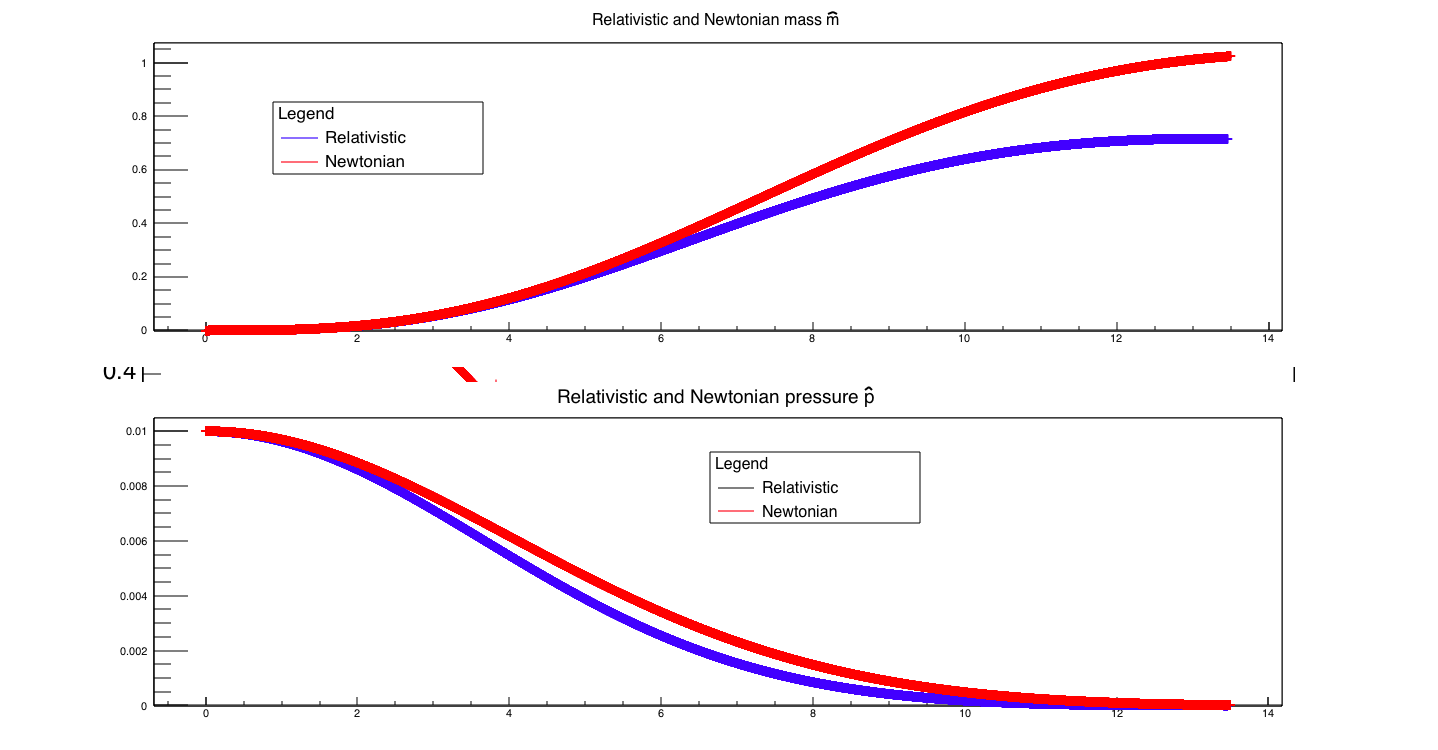
\includegraphics[width=1.1\textwidth]{3_c.png}
\caption{Comparing the pressure and mass of Newtonian and relativistic solution. Unit of mass are in solar mass, unit of radius in km and unit of pressure are in $\epsilon_o$ }
\label{3c}

\end{figure}
\FloatBarrier
\paragraph{}
Referring to Figure \ref{3c}, the Newtonian mass increases faster than the relativistic one. That means a higher average density, consistent with larger pressure shown in the second graph.
\paragraph{}
All the corrections in TOV equations are greater than 1 and strengthen gravitational interaction, consequently put a stronger constraint on maximum mass within a radius (to not form a black hole) , as shown on Figure \ref{3c}

\subsection{Finding for $\hat{M}$ and $\hat{R}$}


\begin{figure}[!htpb]
\begin{center}
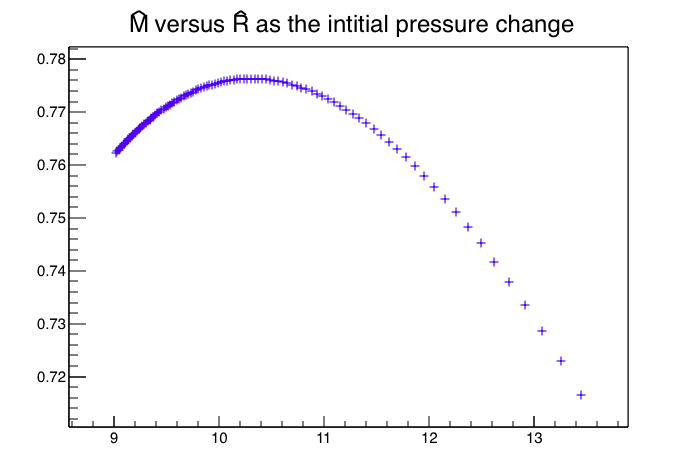
\includegraphics[width=0.8\textwidth]{3_d.png}
\caption{ $\hat{M}$ and $\hat{R } $ are solved for 100 points of initial pressure between 0.01 and 1.1. From left to right, the initial pressure decreases}
\label{3d}
\end{center}
\end{figure}
\FloatBarrier
\paragraph{}
The $\hat{M}$-$\hat{R}$ plot is shown in Figure \ref{3d}. Clearly, there is a maximum for the mass. To find out, as in problem 1 and 2, three nearest points to the maximum mas was fitted to a quadratic and the maximum was found by setting the first derivative of the quadratic equal to zero. The result is $\hat{M}_{max} $=0.776339 solar mass and $\hat{R}$=10.3064km. These are close to famous result from Oppenheimer and Volkow 1939.


\begin{thebibliography}{9}
\bibitem{Beck}
  Fowles and Cassiday,
  \emph{Analytical Mechanics}

\bibitem{Beck}
  Roman Scoccimarro
  \emph{Lecture notes}
  
\end{thebibliography}
\end{document}


